\chapter{Tipos de dados Especiais}
Neste capítulo veremos alguns tipos de dados especiais que o MDArte implementa e
como utilizá-los, a fim de facilitar a comunicação com o banco de dados e o
tratamento dos dados da aplicação.

\section{Hstore}
O hstore é um tipo de dados disponível no Postgres que permite, para uma mesma
coluna de uma linha na tabela, relacionar valores de texto à chaves, que também
são textos, tal qual um Map em Java.
Para mais informações sobre o funcionamento do hstore, consulte
http://www.postgresql.org/docs/9.4/static/hstore.html.
Nesta seção veremos como utilizar o tipo hstore nas entitades de um sistema
desenvolvido com o MDArte.

\subsection{Criando um atributo com o tipo hstore}
No diagrama de classes da sua camada de domínio, abra a especificação do
atributo que deverá ser do tipo hstore. No campo type, selecione o tipo Hstore,
como na imagem abaixo:
\begin{figure}[H]
	\centering
	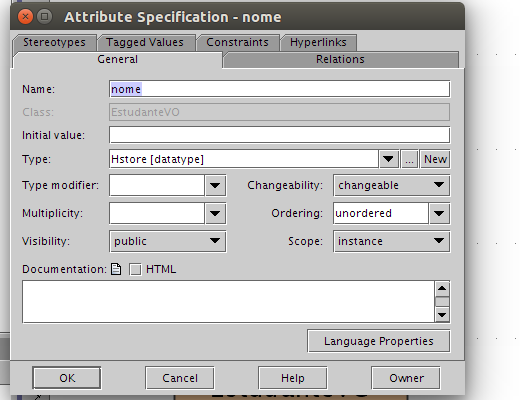
\includegraphics[width=290pt,height=220pt]{files/imgs/hstore-0000.png}
	\caption{Configuração do parâmetro matrícula da classe Estudante.}
	\label{config_parametro}
\end{figure}

O resultado na classe que representa a entidade, será o seguinte:
\begin{figure}[H]
	\centering
	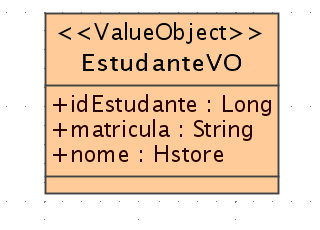
\includegraphics[width=260pt,height=180pt]{files/imgs/hstore-0001.png}
	\caption{Entidade com o atributo nome já com o tipo hstore.}
	\label{config_parametro}
\end{figure}

Feito isto, vá na pasta raiz do projeto e regere o mesmo usando o comando \texttt{maven}. O \texttt{MDArte irá então regerar as classes da camada de domínio, bem como os \texttt{scripts SQL} corrspondentes aos novos atributos da entidade. Você provavelmente precisará rodar novamente o \texttt{script schema-create.sql}, ou alterar manualmente a tabela, a fim de que o atributo escolhido como \texttt{hstore} tem a tipagem correta na tabela do banco. Você provavelmente precisará também reinserir os dados da sua aplicação, caso a tabela já tenha alguma informação. 
